\documentclass[11pt]{article}
\usepackage{latexsym}
\usepackage{amsmath,fullpage,amsthm,fancyhdr,amsfonts,amssymb}
\usepackage[svgnames]{xcolor}
\usepackage{graphicx}
\usepackage{float}
\usepackage{import, pst-plot}
\def\emptyline{\vspace{12pt}}

\usepackage{caption}
\usepackage{subcaption}



\pagestyle{fancy}
\lhead{ AMATH 574}
\chead{Monday}
\rhead{Student ID: 1111111}
\lfoot{}
\cfoot{\thepage}
\rfoot{}
\renewcommand{\headrulewidth}{0.1pt}
\renewcommand{\footrulewidth}{0.1pt}
\setlength{\textwidth}{6.2in}
\setlength{\textheight}{8.7in}
\setlength{\voffset}{-.7in}
\setlength{\headsep}{26pt}
\setlength{\parindent}{10pt}

\begin{document}

\title{\Large\bf Homework 3}
\author{Monday}
\date{due date: \today}
\maketitle
\thispagestyle{fancy}
\renewcommand{\qed}{\hfill \mbox{\raggedright \rule{0.07in}{0.1in}}} % for the use of end of proof mark

\begin{enumerate}
%-------------------------------------------------------------------------------------
%---Problem \#11.2 -------------------------------------------------------------------
    \item Problem \#11.2
            
			Show that the viscous Burgers equation $u_t+uu_x=\epsilon u_{xx}$ has a travelling-wave solution of the form $u^{\epsilon}(x,t)=w^{\epsilon}(x-st)$, by deriving an ODE for $w$ and verifying that this ODE has solutions of the form
			\[
			w(\xi)=u_r+\frac{1}{2}(u_l-u_r)[1-\tanh(\frac{(u_l-u_r)\xi}{\epsilon})]
			\]
			where $u_l>u_r$, with the propagation speed $s$ agreeing with the shock speed $s=\frac{1}{2}(u_l+u_r)$. Note that $w(\xi)\rightarrow u_l$ as $\xi\rightarrow -\infty$, and $w(\xi)\rightarrow u_r$ as $\xi \rightarrow +\infty$. Sketch this solution and indicate how it varies as $\epsilon \rightarrow 0$. What happens to this solution if $u_l<u_r$, and why is there no traveling-wave solution with limiting values of this form?
		
		\vskip 5pt
        \noindent{\bf Solution}
        \vskip 5pt
        
        	Assume viscous Burgers equation has a travelling wave solution of the form 
        	\[
        	u^{\epsilon}(x,t)=w^{\epsilon}(x-st)
        	\]	
        	Substitute $w^{\epsilon}$ into viscous Burgers equation
        	\[
        	\Rightarrow -s(w^{\epsilon})'+w^{\epsilon}(w^{\epsilon})'=\epsilon(w^{\epsilon})''
        	\]
        	Now we can check if $w(\xi)$ satisfy this ODE
        	\begin{align*}
        	w'(\xi)&=-\frac{(u_l-u_r)^2}{8\epsilon}[1-\tanh^2(\frac{(u_l-u_r)\epsilon}{4\epsilon})]\\
        	w''(\xi)&=\frac{(u_l-u_r)^3}{16\epsilon^2}\tanh(\frac{(u_l-u_r)\epsilon}{4\epsilon})[1-\tanh^2(\frac{(u_l-u_r)\epsilon}{4\epsilon})]
        	\end{align*}
        	Plug the above results in left hand side of ODE, (denote$\frac{(u_l-u_r)\epsilon}{4\epsilon}=\theta$)
        	\begin{align*}
        	-s(w^{\epsilon})'+w^{\epsilon}(w^{\epsilon})'
        	= & \frac{s}{8\epsilon}(u_l-u_r)^2[1-\tanh^2(\theta)]-\frac{1}{8\epsilon}u_r(u_r-u_l)^2[1-\tanh^2(\theta)]\\
        	& -\frac{1}{16\epsilon}(u_l-u_r)^3[1-\tanh(\theta)][1-\tanh^2(\theta)]\\
        	= & \frac{s}{8\epsilon}(u_l-u_r)^2[1-\tanh^2(\theta)]-\frac{1}{16\epsilon}(u_l+u_r)(u_r-u_l)^2[1-\tanh^2(\theta)]\\
        	& \frac{1}{16\epsilon}(u_l-u_r)^3\tanh(\theta)[1-\tanh^2(\theta)]
        	\end{align*}
        	Right hand side of ODE
        	\begin{align*}
        	\epsilon(w^{\epsilon})''=\frac{1}{16\epsilon}(u_l-u_r)^3\tanh(\theta)[1-\tanh^2(\theta)]
        	\end{align*}
        	If we let $LHS=RHS$, then
        	\[
        	\frac{s}{8\epsilon}(u_l-u_r)^2[1-\tanh^2(\theta)]-\frac{1}{16\epsilon}(u_l+u_r)(u_r-u_l)^2[1-\tanh^2(\theta)]=0
        	\]
        	\[
        	\Rightarrow s=\frac{1}{2}(u_r+u_l)
        	\]
        	Thus we have verified that if the propagation speed $s$ agrees with shock speed $\frac{1}{2}(u_r+u_l)$, then the travelling wave solution is a solution of ODE derived by Burgers equation.
        	
        	Assume in the same moving frame with speed $s$, the profile of $w$ tends to form a shock at the origin.
        	
        	\hfil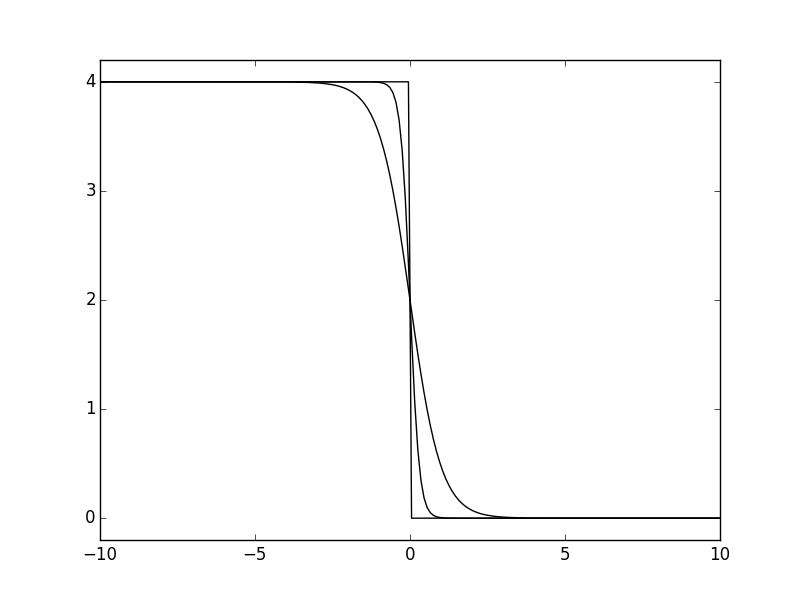
\includegraphics[width=4.0in]{problem_11_2.png}\hfil
        	
        	For the case $u_l<u_r$
        	\begin{align*}
        	w(\xi)\rightarrow u_r \text{ as } \xi\rightarrow -\infty \\
        	w(\xi)\rightarrow u_l \text{ as } \xi\rightarrow +\infty
        	\end{align*}
        	That would violate the assumption about value of $w$ as $\xi$ goes to $\infty$.
        	        	
\qed
\newpage  

%-------------------------------------------------------------------------------------        
%---Problem \#11.3 --------------------------------------------------------------------
    \item Problem \#11.3
    
			For a general smooth scalar flux functions $f(q)$, show by Taylor expansion of 
			\[
			s=\frac{f(q_r)-f(q_l)}{q_r-q_l}
			\]			 
			that the shock speed is approximately the average of the characteristic speed on each side,
			\[
			s=\frac{1}{2}[f'(q_l)+f'(q_r)]+\mathcal{O}(|q_r-q_l|^2)
			\] 
    
		\vskip 5pt
        \noindent{\bf Solution}
        \vskip 5pt
			
			Assume flux function $f(q)$ is smooth enough that the following Taylor expansion is valid.
			
			First, Taylor expansion $f(\frac{q_l+q_r}{2})$ at $q_r$
			\[
			f(\frac{q_l+q_r}{2})=f(q_r)+f'(q_r)\frac{1}{2}(q_l-q_r)+\frac{f''(q_r)}{2}[\frac{1}{2}(q_l-q_r)]^2+\mathcal{O}(|q_r-q_l|^3)
			\]
			\[
			\Rightarrow 
			f(q_r) = f(\frac{q_l+q_r}{2})-f'(q_r)\frac{1}{2}(q_l-q_r)-\frac{f''(q_r)}{2}[\frac{1}{2}(q_l-q_r)]^2+\mathcal{O}(|q_r-q_l|^3)
			\]
			Then, Taylor expansion $f(\frac{q_l+q_r}{2})$ at $q_l$
			\[
			f(\frac{q_l+q_r}{2})=f(q_l)+f'(q_l)\frac{1}{2}(q_r-q_l)+\frac{f''(q_l)}{2}[\frac{1}{2}(q_r-q_l)]^2+\mathcal{O}(|q_r-q_l|^3)
			\]
			\[
			\Rightarrow 
			f(q_l)=f(\frac{q_l+q_r}{2})-f'(q_l)\frac{1}{2}(q_r-q_l)-\frac{f''(q_l)}{2}[\frac{1}{2}(q_r-q_l)]^2+\mathcal{O}(|q_r-q_l|^3)
			\]
			Substitute $f(q_r)$ and $f(q_l)$ into $s=\frac{f(q_r)-f(q_l)}{q_r-q_l}$
			\begin{align*}
			s=&\frac{1}{q_r-q_l}[f(\frac{q_l+q_r}{2})-f'(q_r)\frac{1}{2}(q_l-q_r)-\frac{f''(q_r)}{2}[\frac{1}{2}(q_l-q_r)]^2+\mathcal{O}(|q_r-q_l|^3)\\
			&-f(\frac{q_l+q_r}{2})+f'(q_l)\frac{1}{2}(q_r-q_l)+\frac{f''(q_l)}{2}[\frac{1}{2}(q_r-q_l)]^2+\mathcal{O}(|q_r-q_l|^3)]\\
			=&\frac{f'(q_r)+f'(q_l)}{2} + \frac{1}{8}[f''(q_l)-f''(q_r)](q_r-q_l)+\mathcal{O}(|q_r-q_l|^2)
			\end{align*}
			Do another Taylor expansion of term $\frac{1}{8}[f''(q_l)-f''(q_r)](q_r-q_l)$ in the above expression to show that it is actually $\mathcal{O}(|q_r-q_l|^2)$
			\begin{align*}
			f''(q_l)-f''(q_r) = f'''(q_r)(q_l-q_r)+\mathcal{O}(|q_l-q_r|^2)
			\end{align*}
			Thus 
			\[
			\frac{1}{8}[f''(q_l)-f''(q_r)](q_r-q_l)=\mathcal{O}(|q_r-q_l|^2)
			\]
			Now we can get
			\[
			s=\frac{f'(q_r)+f'(q_l)}{2}+\mathcal{O}(|q_r-q_l|^2)
			\]

\qed
\newpage  

%-------------------------------------------------------------------------------------        
%---Problem \#11.8 --------------------------------------------------------------------
    \item Problem \#11.8
    		Consider the scalar conservation law $u_t+(e^u)_x=0$. Determine the exact solution with the following sets of initial data:
    		\begin{enumerate}   		
			\item	
			\[\mathring{u}=\begin{cases}1\text{  if }x<0\\0\text{  if }x>0\end{cases}\] 				\item
			\[\mathring{u}=\begin{cases}0\text{  if }x<0\\1\text{  if }x>0\end{cases}\] 
			\item
			\[\mathring{u}=\begin{cases}2\text{  if }0<x<1\\0\text{  otherwise}\end{cases}\]  		
    		\end{enumerate}
    
		\vskip 5pt
        \noindent{\bf Solution}
        \vskip 5pt
			
			Characteristics for this scalar conservation law problem
			\[
			x'(t)=f'(u), \text{ where } f'(u)=e^u
			\]
			\begin{enumerate}
			
			\item
				\begin{align*}
				\text{For } x<0,\ x'(t)=e^1=e\\
				\text{For } x>0,\ x'(t)=e^0=1
				\end{align*}	
				\hfil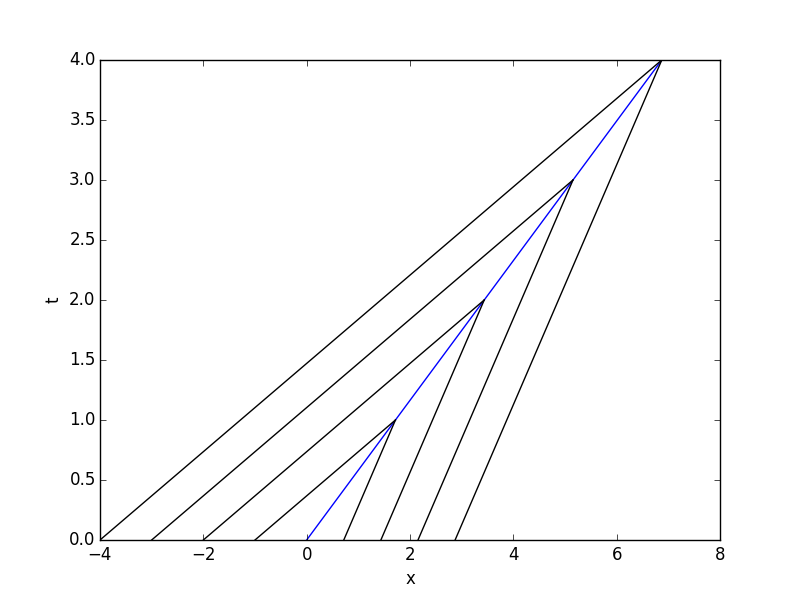
\includegraphics[width=3.0in]{problem_11_8a_char.png}\hfil
				
				From the characteristic structure we can tell shock forms at $t=0$, $x=0$. Then by Rankine-Hugoniot condition, shock speed can be derived for this scalar conservation law.
				\[
				s = \frac{f(u_r)-f(u_l)}{u_r-u_l}=e-1
				\]
				Thus the location of shock in the $x-t$ plane is
				\[
				x_s(t)=(e-1)t
				\]			
				And the solution for all $x$, $t$ is 
				\[
				u(x,t)=\begin{cases}1, \ x<(e-1)t \\ 0, \ x>(e-1)t \end{cases}
				\]
				About the plots of solution at several instants in time, it should be the same profile as initial with moving speed equals $s$. 
				
				\hfil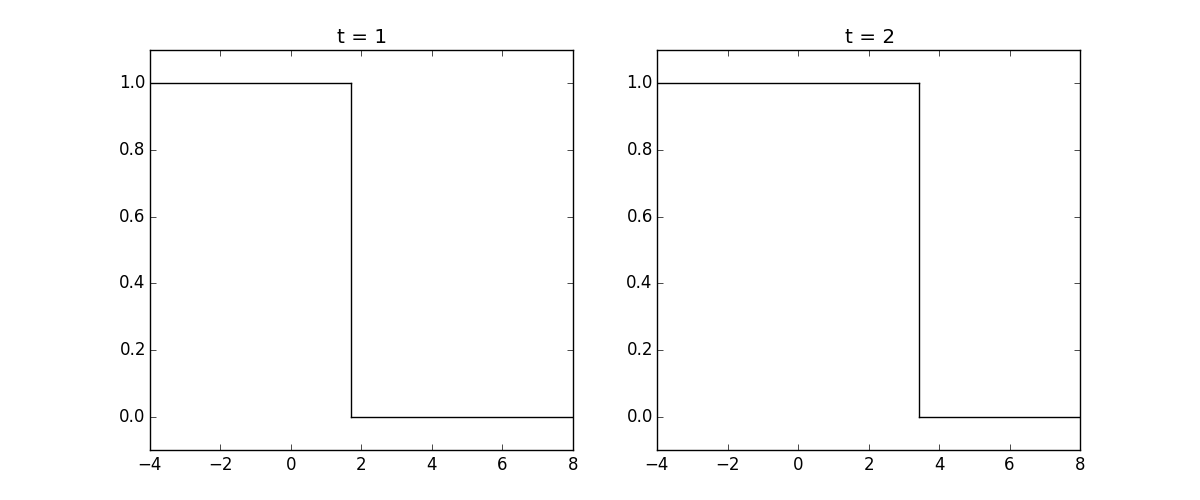
\includegraphics[width=6.0in]{problem_11_8a.png}\hfil
				
				I try to modify "burgers" to see the results. But it seems like I should use a different boundary condition in order to get the right plots. That would result in changing clawdata.bclower[0] = 'user' in setrun.py, I think. The file "bcNamr.f" is supposed to be inside directory "CLAW/amrclaw/src/Nd/bcNamr.f", which turns out is not the case. "CLAW/amrclaw/src" only have 2D and 3D cases.
			\item
				\begin{align*}
				\text{For } x<0,\ x'(t)=e^0=1\\
				\text{For } x>0,\ x'(t)=e^1=e
				\end{align*}
				\hfil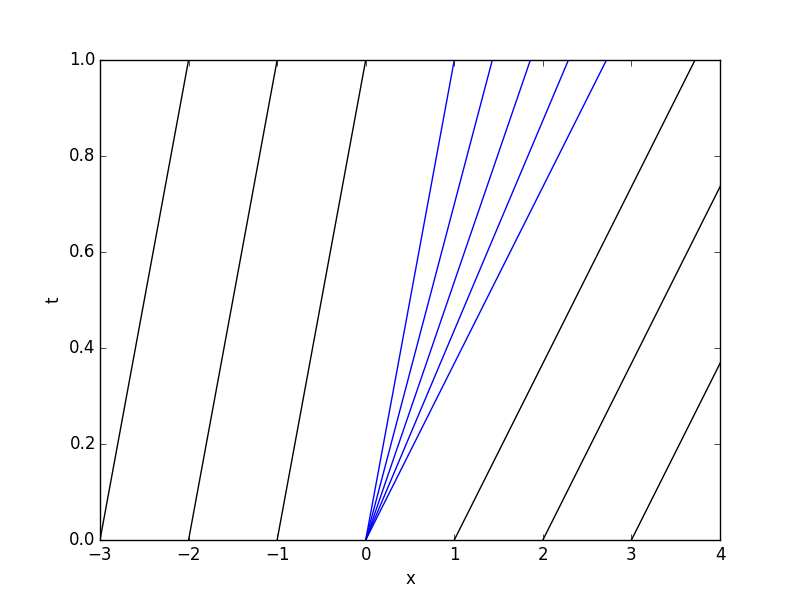
\includegraphics[width=3.0in]{problem_11_8b_char.png}\hfil	
				
				From the characteristic structure we can tell rarefaction fan forms at $t=0$, $x=0$. Then we can find similarity solution by assuming $u(x,t)=\tilde{u}(x/t)$.
				\[
				-\frac{x}{t^2}\tilde{u}'+e^{\tilde{u}}\tilde{u}'\frac{1}{t}=0
				\]
				Thus the value of $u$ inside rarefaction fan is 
				\[
				\tilde{u}(x/t)=\ln(x/t)
				\]			
				And the solution for all $x$, $t$ is 
				\[
				u(x,t)=\begin{cases}0, \ x<t \\ 1, \ x>et\\ \ln(x/t), \ t<x<et \end{cases}
				\]
				The following are plots of solution at several instants in time
				
				\hfil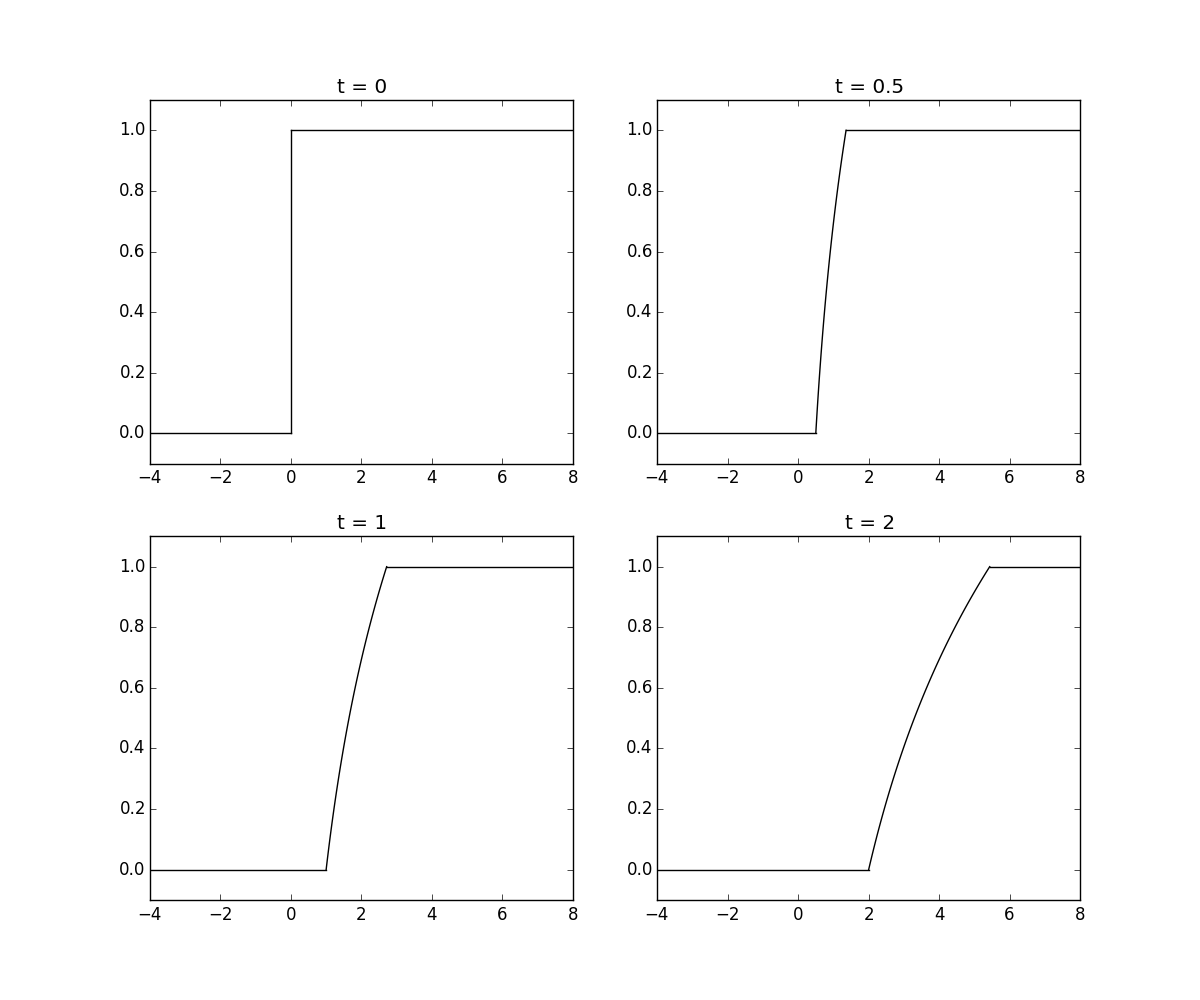
\includegraphics[width=6.0in]{problem_11_8b.png}\hfil
				
				When try to use CLAWPACK to verify the result, I came across the same problem as in (a). Periodic boundary condition won't give the right figure.
				
			\item
				\begin{align*}
				&\text{For } x<0, \ x'(t)=e^0=1\\
				&\text{For } 0<x<1, \ x'(t)=e^2=e^2\\
				&\text{For } x>1, \ x'(t)=e^0=1
				\end{align*}
				From the characteristic structure

				\hfil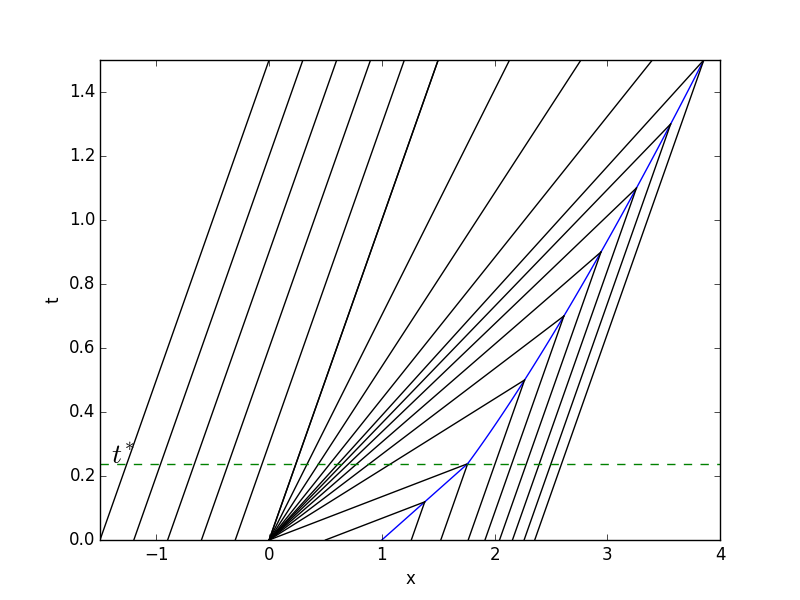
\includegraphics[width=3.0in]{problem_11_8c_char.png}\hfil
			
				At time $t=0$ 
				\begin{align*}
				& t=0, x=0, \text{ rarefaction fan}\\
				& t=0, x=1, \text{ shock}
				\end{align*}
				\begin{align*}
				&\text{rarefaction fan: } \tilde{u}(x/t)=\ln(x/t)\\
				&\text{shock: } s=\frac{f(u_r)-f(u_l)}{u_r-u_l}=\frac{1}{2}(e^2-1)
				\end{align*}
				At some later time, rarefaction fan will hit shock. The starting point can be derived from the following system
				\[
				\begin{cases}
				x=e^2t\\
				x=1+\frac{1}{2}(e^2-1)t
				\end{cases}
				\]
				At time $t^*=\frac{2}{e^2+1}$, a new shock forms. Values on left side has changed to values inside rarefaction fan. The speed of shock is no longer constant.
				\[
				x'(t)=s=\frac{f(u_l)-f(u_r)}{u_l-u_r}=\frac{x/t-1}{\ln(x/t)}
				\]
				Solve this ODE numerically would give the shock location in $x-t$ plane.\\
				
				The following is solution
				\begin{align*}
				&t\leq\frac{2}{e^2+1},\ 
				u(x,t)=\begin{cases}0, \ &x<t\\ \ln(x/t), \ &t<x<e^2t\\ 2, \ &e^2t<x<1+\frac{1}{2}(e^2-1)t\\ 0, \ &1+\frac{1}{2}(e^2-1)t<x\end{cases}\\
				&t>\frac{2}{e^2+1}, \
				u(x,t)=\begin{cases}0, \ &x<t\\ \ln(x/t), \ &t<x<\tilde{x}(t)\\ 0,,\ &\tilde{x}(t)<x\end{cases}
				\end{align*}
				Here $\tilde{x}(t)$ stands for the location of shock after $\frac{2}{e^2+1}$. The following gives the explicit expression of $\tilde{x}(t)$.\\
				
				We may use Equal-Area Rule to determine the location of shock, which would result in the following figure. Since it is the relation between one time instant and another, we can assume the position of shock after some time period. Then use the Equal-Area Rule to find the equation that the position should satisfy.\\
				
				\hfil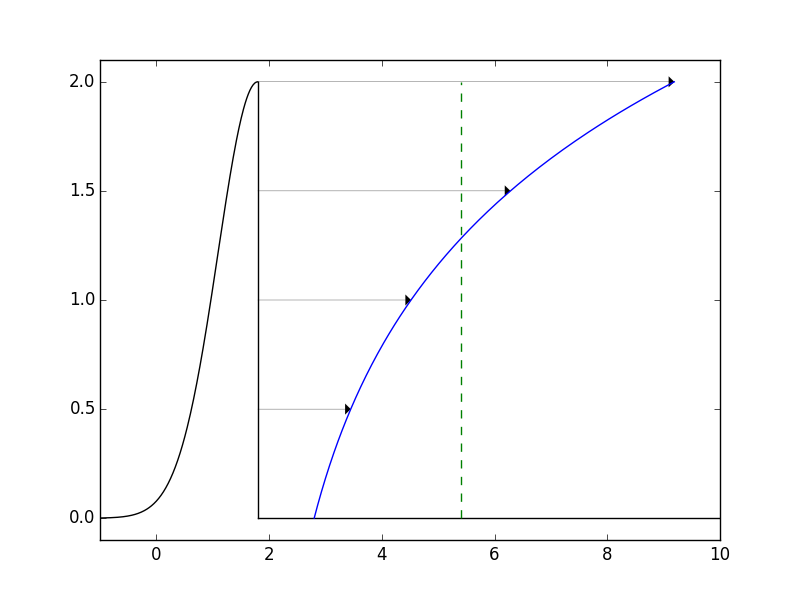
\includegraphics[width=3.0in]{problem_11_8c.png}\hfil \\
				
				The green line stands for the position after some time period. The above figure is just the relation when time interval is very small. The long time behaviour should be captured by using the value from the left rarefaction fan.\\
				
				We need to know the profile of triple valued function for each point along x axis. And then we can do integration. The left edge would be rarefaction fan with value $ \ln(x/t) $. The long time profile should look like the following\\
				
				\hfil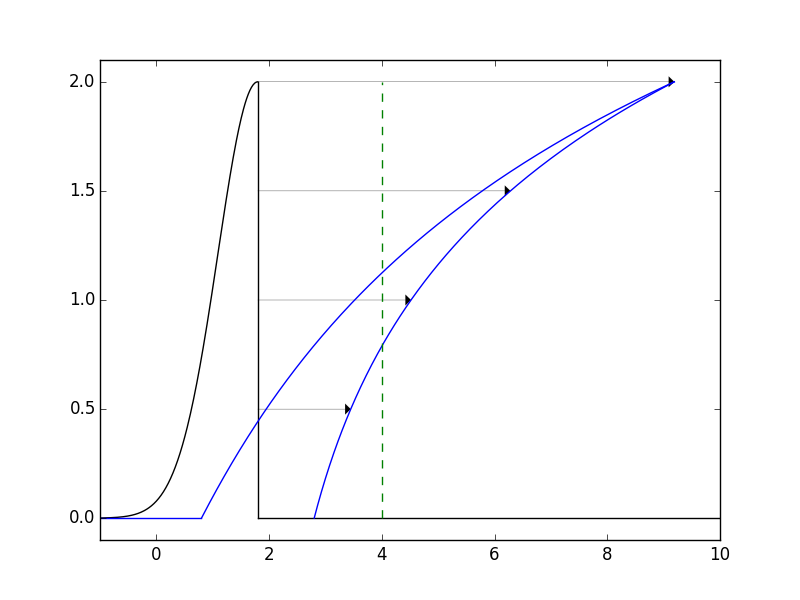
\includegraphics[width=3.0in]{problem_11_8c_long.png}\hfil\\
				
				Suppose the profile can be cut by green line above, and still result in the same area. Then we can get the following integral:
				\[
				\int_t^{\tilde{x}} \ln(s/t)ds = 2
				\]
				Thus we can get $\ln(\tilde{x}/t)\tilde{x}-\tilde{x}+t=2$. This is the equation that shock position should satisfy after $t^*$. 
			\end{enumerate}
\qed
\newpage  

%-------------------------------------------------------------------------------------        
%---Problem \#13.1 --------------------------------------------------------------------
    \item Problem \#13.1
    		\begin{enumerate}
    			\item
    				Consider an integral curve of $r^1$ for the shallow water equations. Show that the slope tangent to this curve in the $q^1-q^2$ plane at any point is equal to $\lambda^1$ at the point. ($q^1=h$ and $q^2=hu$.)
    			\item
    				Consider the Hugoniot locus for 1-shocks for the shallow water equations. Show that if $q_l$ and $q_l$ are two points lying on this curve (and hence connected by a 1-shock) then the slope of the secant line connecting these points is equal to the shock speed $s$.
    		\end{enumerate} 
    		    
		\vskip 5pt
        \noindent{\bf Solution}
        \vskip 5pt
        	
        	\begin{enumerate}
        		\item
        			Under some particular parametrization, the integral curve can be determined by the following differential equations
        			\begin{align*}
        			\tilde{q}'(\xi)=r^1(\tilde{q}(\xi))=\begin{bmatrix}1\\ \tilde{q}^2/\tilde{q}^1-\sqrt{g\tilde{q}^1}\end{bmatrix}
        			\end{align*}
        			At point $q^1=h$, $q^2=hu$.
        			\begin{align*}
        			&dq^1=d\xi,\\
        			&dq^2=(u-\sqrt{gh})d\xi
        			\end{align*}
        			From this we can derive the slope tangent to this integral curve at this point, which is 
        			\[
        			\frac{dq^2}{dq^1}=u-\sqrt{gh}=\lambda^1
        			\]
        		\item
        			If $q_l$ and $q_r$ are two points lying on this curve, then these two states can be connected by a shock satisfying Rankine-Hugoniot conditions, which means 
        			\[
        			s(q_r-q_l)=f(q_r)-f(q_l)
        			\]
        			For the shallow water equations, this gives a system of two equations that must be satisfied:
        			\begin{align*}
        			s(h_r-h_l)&=h_ru_r-h_lu_l\\
        			s(h_ru_r-h_lu_l)&=h_ru_r^2-h_lu_l^2+\frac{1}{2}g(h_r^2-h_l^2)
        			\end{align*}
        			Then from the first equation
        			\[
        			s=\frac{h_ru_r-h_lu_l}{h_r-h_l}
        			\]
        			which means the slope of the secant line connecting these points is equal to the shock speed $s$
        	\end{enumerate}
\qed
\newpage  

%-------------------------------------------------------------------------------------        
%---Problem \#13.7 --------------------------------------------------------------------
    \item Problem \#13.7
    		Consider the p-system 
    		\begin{align*}
    		v_t-u_x&=0,\\
    		u_t+p(v)_x&=0,
    		\end{align*}
    		where $p(v)$ is a given function of $v$.
    		\begin{enumerate}
    		\item
    			Compute the eigenvalues of the Jacobian matrix, and show that the system is hyperbolic provided $p'(v)<0$.
    		\item
    			Use the Rankine-Hugoniot condition to show that a shock connecting $q=(v,u)$ to some fixed state $q^*=(v_*,u_*)$ must satisfy 
    			\[
    			u=u_*\pm\sqrt{-(\frac{p(v)-p(v_*)}{v-v_*})}(v-v_*)
    			\]
    		\item
    			What is the propagation speed for such a shock? How does this relate to the eigenvalues of the Jacobian matrix computed in part (a)?
    		\item
    			Plot the Hugoniot loci for the point $q_*=(1,1)$ over the range $-3\leq v\leq 5$ for the following $p(v)$
    			\[
    			p(v)=-e^v
    			\]
    		\end{enumerate}
      		    
		\vskip 5pt
        \noindent{\bf Solution}
        \vskip 5pt
        	
        	\begin{enumerate}
        		\item
        			The equations can be written as a linear system
        			\[
        			\begin{bmatrix}v\\u\end{bmatrix}_t+
        			\begin{bmatrix}0&-1\\p'(v)&0\end{bmatrix}
        			\begin{bmatrix}v\\u\end{bmatrix}_x=0
        			\]
        			\[
        			A=\begin{bmatrix}0&-1\\p'(v)&0\end{bmatrix}
        			\]
        			If $p'(v)<0$, then $|\lambda I-A|=\lambda^2+p'(v)=0$ has two different real eigenvalues. Thus this system is hyperbolic.
        		\item
        			By Rankine-Huguniot condition, the followings must be satisfied 
        			\begin{align*}
        			s(v_*-v)&=-u_*+u\\
        			s(u_*-u)&=p(v_*)-p(v)
        			\end{align*}  
        			\[
        			\Rightarrow -\frac{(u-u_*)^2}{v_*-v}=p(v_*)-p(v)
        			\]
        			Thus
        			\[
        			u-u_*=\pm\sqrt{-(\frac{p(v)-p(v_*)}{v-v_*})}(v-v_*)
        			\]
        		\item
        			From Rankine-Huguniot condition in (b), we can also eliminate $u$, which would give
        			\[
        			s^2=-\frac{p(v_*)-p(v)}{v_*-v}
        			\]
        			Thus $s=\pm\sqrt{-\frac{p(v_*)-p(v)}{v_*-v}}$. As $v_*\rightarrow v$, $s\rightarrow \pm\sqrt{-p'(v)}$.
        		\item
        			As we have discussed in (b), let $p(v)=-e^v$.
        			
        			\hfil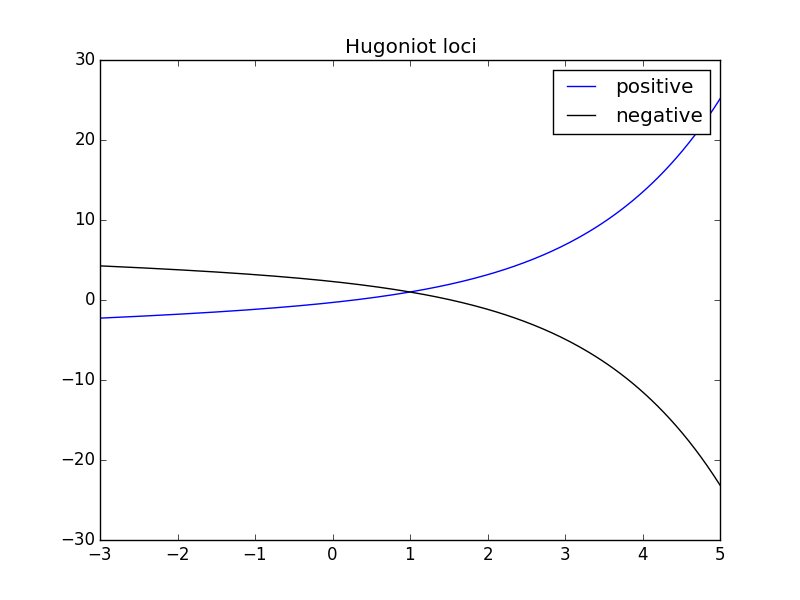
\includegraphics[width=3.0in]{problem_13_7.png}\hfil

        	\end{enumerate}
\qed

\end{enumerate}

\end{document}